\documentclass[11pt]{article}

\usepackage[portuguese]{babel}
\usepackage[utf8]{inputenc}
\usepackage{amsmath}
\usepackage{graphicx}
\usepackage{float}
\usepackage{subfig}
\usepackage{fixltx2e}
\usepackage[bottom]{footmisc}
\usepackage{color}
\usepackage{xargs}                      % Use more than one optional parameter in a new commands
\usepackage[pdftex,dvipsnames]{xcolor}  % Coloured text etc.
\usepackage[colorinlistoftodos,prependcaption,textsize=tiny]{todonotes}
\newcommandx{\unsure}[2][1=]{\todo[linecolor=red,backgroundcolor=red!25,bordercolor=red,#1]{#2}}
\newcommandx{\change}[2][1=]{\todo[linecolor=blue,backgroundcolor=blue!25,bordercolor=blue,#1]{#2}}
\newcommandx{\info}[2][1=]{\todo[linecolor=OliveGreen,backgroundcolor=OliveGreen!25,bordercolor=OliveGreen,#1]{#2}}
\newcommandx{\improvement}[2][1=]{\todo[linecolor=Plum,backgroundcolor=Plum!25,bordercolor=Plum,#1]{#2}}
\newcommandx{\thiswillnotshow}[2][1=]{\todo[disable,#1]{#2}}
\usepackage[font=footnotesize]{caption}

\numberwithin{equation}{section}

\linespread{1.3}
\usepackage{indentfirst}
\usepackage[top=2cm, bottom=2cm, right=2.25cm, left=2.25cm]{geometry}
\addto\captionsportuguese{\renewcommand{\contentsname}{Índice}}

\begin{document}

\begin{titlepage}
\begin{center}

\hfill \break
\hfill \break


\includegraphics[width=0.3\textwidth]{./logo}~\\[1cm]

\textsc{\LARGE Instituto Superior Técnico}\\[0.25cm]
\textsc{\Large Mestrado Integrado em Engenharia Electrotécnica e de Computadores}\\[1.8cm]
\textsc{\huge Sistemas Integrados Analógicos}\\[0.25cm]

{\huge \bfseries \textit{Design} de um Amplificador \\[0.2cm]
				Errata\\[2cm]}

\begin{tabular}{ l l }
João Bernardo Sequeira de Sá & \hspace{2mm} n.º 68254 \\
Maria Margarida Dias dos Reis & \hspace{2mm} n.º 73099 \\
Nuno Miguel Rodrigues Machado & \hspace{2mm} n.º 74236
\end{tabular}

\vfill

{\large Lisboa, 3 de Maio de 2015} 

\end{center}
\end{titlepage}

\pagenumbering{gobble}
\clearpage

\tableofcontents
\pagebreak

\clearpage
\pagenumbering{arabic}

\section{Errata}

\subsection{Introdução}

Este capítulo foi acrescentado ao relatório final no intuito de corrigir os resultados obtidos e apresentados no último relatório, \textit{middle target}. Como referenciado, pretende-se projectar um amplificador \textit{folded cascode} CMOS OTA de dois andares de acordo com as especificações da seguinte tabela.

\begin{table}[H]
	\centering
	\caption{Características do amplificador a projectar.}
	\vspace{-1.5mm}
	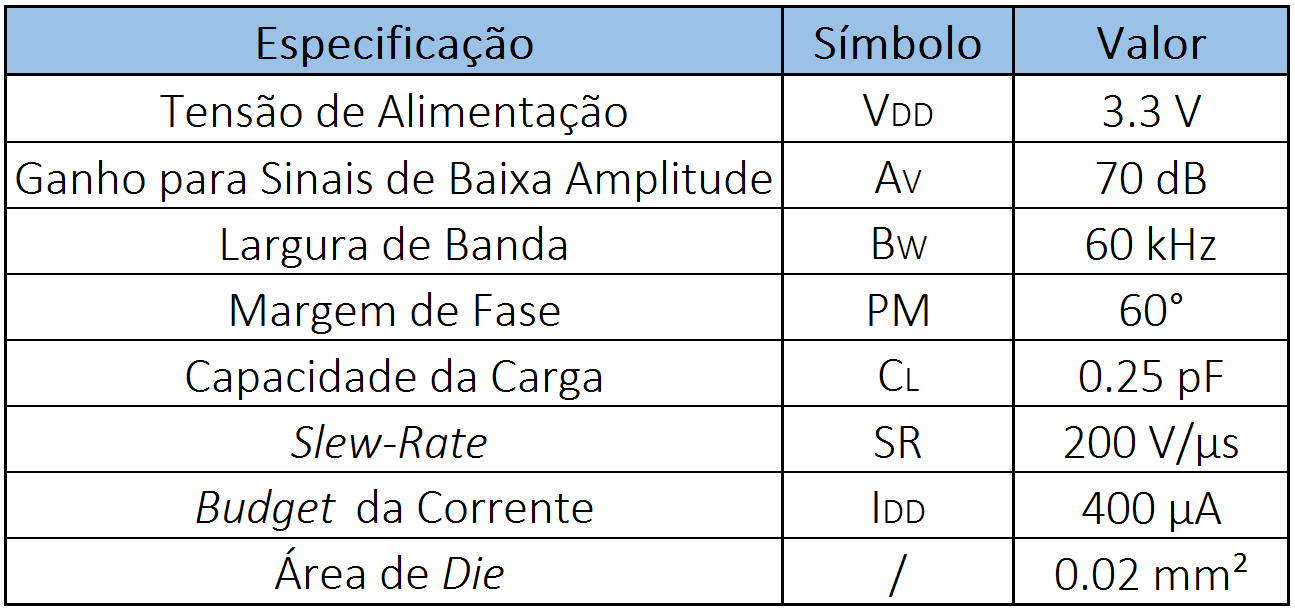
\includegraphics[keepaspectratio=true, scale=0.45]{teoricas/tabela1}
\end{table}


\subsection{Detecção dos erros} 

Foi identificado erros no relatório intermédio que comprometem os resultados apresentados anteriormente. A primeira correcção foi referente ao \textit{schematic} do \textit{testbench} que permite simular o circuito em testes de resposta AC, foi colocado um \textit{switch} que simula a bobine, circuito aberto para um regime AC e curto-circuito para um regime DC. Foi também alterado a amplitude do sinal de entrada de 3.3 V para 1.6 V, esta alteração garante que os transístores não saem da saturação. De seguida pode-se comparar o novo \textit{testbench} com o anterior.

\begin{figure}[H]
	\centering
	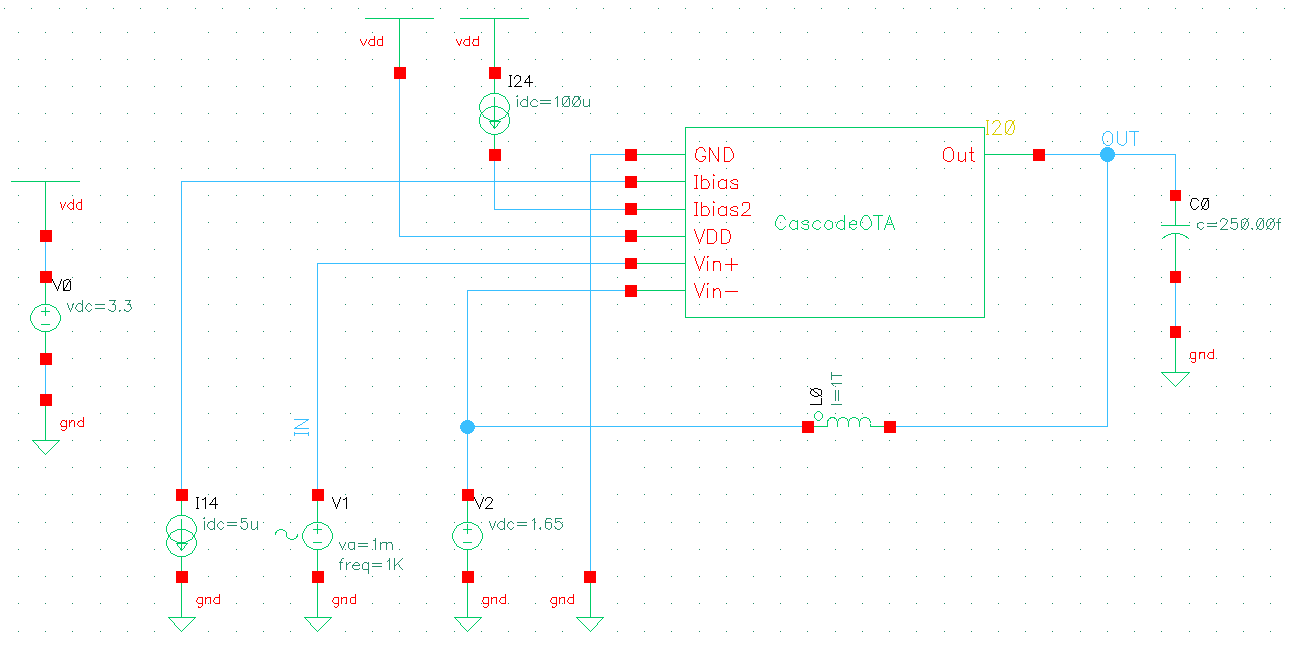
\includegraphics[keepaspectratio=true, scale=0.60]{exps/TBac}
	\vspace{-0.5em}
	\caption{\textit{Schematic} do \textit{testbench} anterior que permite simular o circuito em testes de resposta AC.}
	\vspace{-0.8em}
\end{figure} 

\begin{figure}[H]
	\centering
	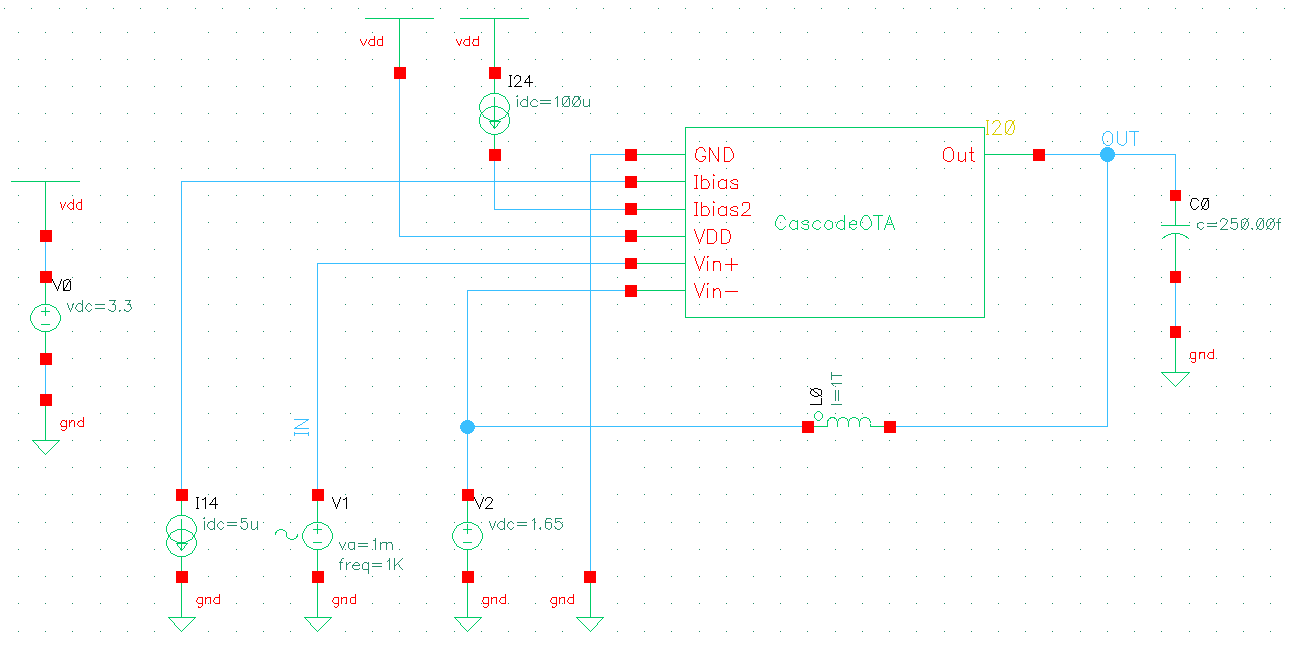
\includegraphics[keepaspectratio=true, scale=0.60]{exps/TBac}
	\vspace{-0.5em}
	\caption{\textit{Schematic} do novo \textit{testbench} anterior que permite simular o circuito em testes de resposta AC.}
	\vspace{-0.8em}
\end{figure} 

Outro erro identificado, foi referente ao calculo da \textit{Slew-Rate}. No relatório intermédio o resultado da \textit{Slew-Rate} era relativo só ao flanco de descida, sendo necessário demonstrar para os dois flancos, subida(1.1) e descida(1.2). De seguida está representado a equação utilizada para o calculo da \textit{Slew-Rate}:

\vspace{-3mm}
\begin{equation}
	slewRate (VT("/OUT") \:\: 1 \:\: nil \:\: 2 \:\: nil \:\: 10 \:\: 90 \:\: nil \:\: "time")
	\label{eq:corrente}
\end{equation}
\vspace{-3mm}
\begin{equation}
	slewRate (VT("/OUT") \:\: 2 \:\: nil \:\: 1 \:\: nil \:\: 10 \:\: 90 \:\: nil \:\: "time")
	\label{eq:corrente}
\end{equation}
\subsection{Correcção do dimensionamento}

 
\subsection{Demonstração de resultados} 

Neste capitulo será representado os resultados do dimensionamento do relatório intermédio e do novo dimensionamento anteriormente referido. 

\subsubsection{Resultados do dimensionamento inicial} 

\subsubsection{Resultados do dimensionamento corrigido} 



\end{document}